\subsection{Class diagram}
The following graphic is the class diagram that we will use for the specification and the implementation.
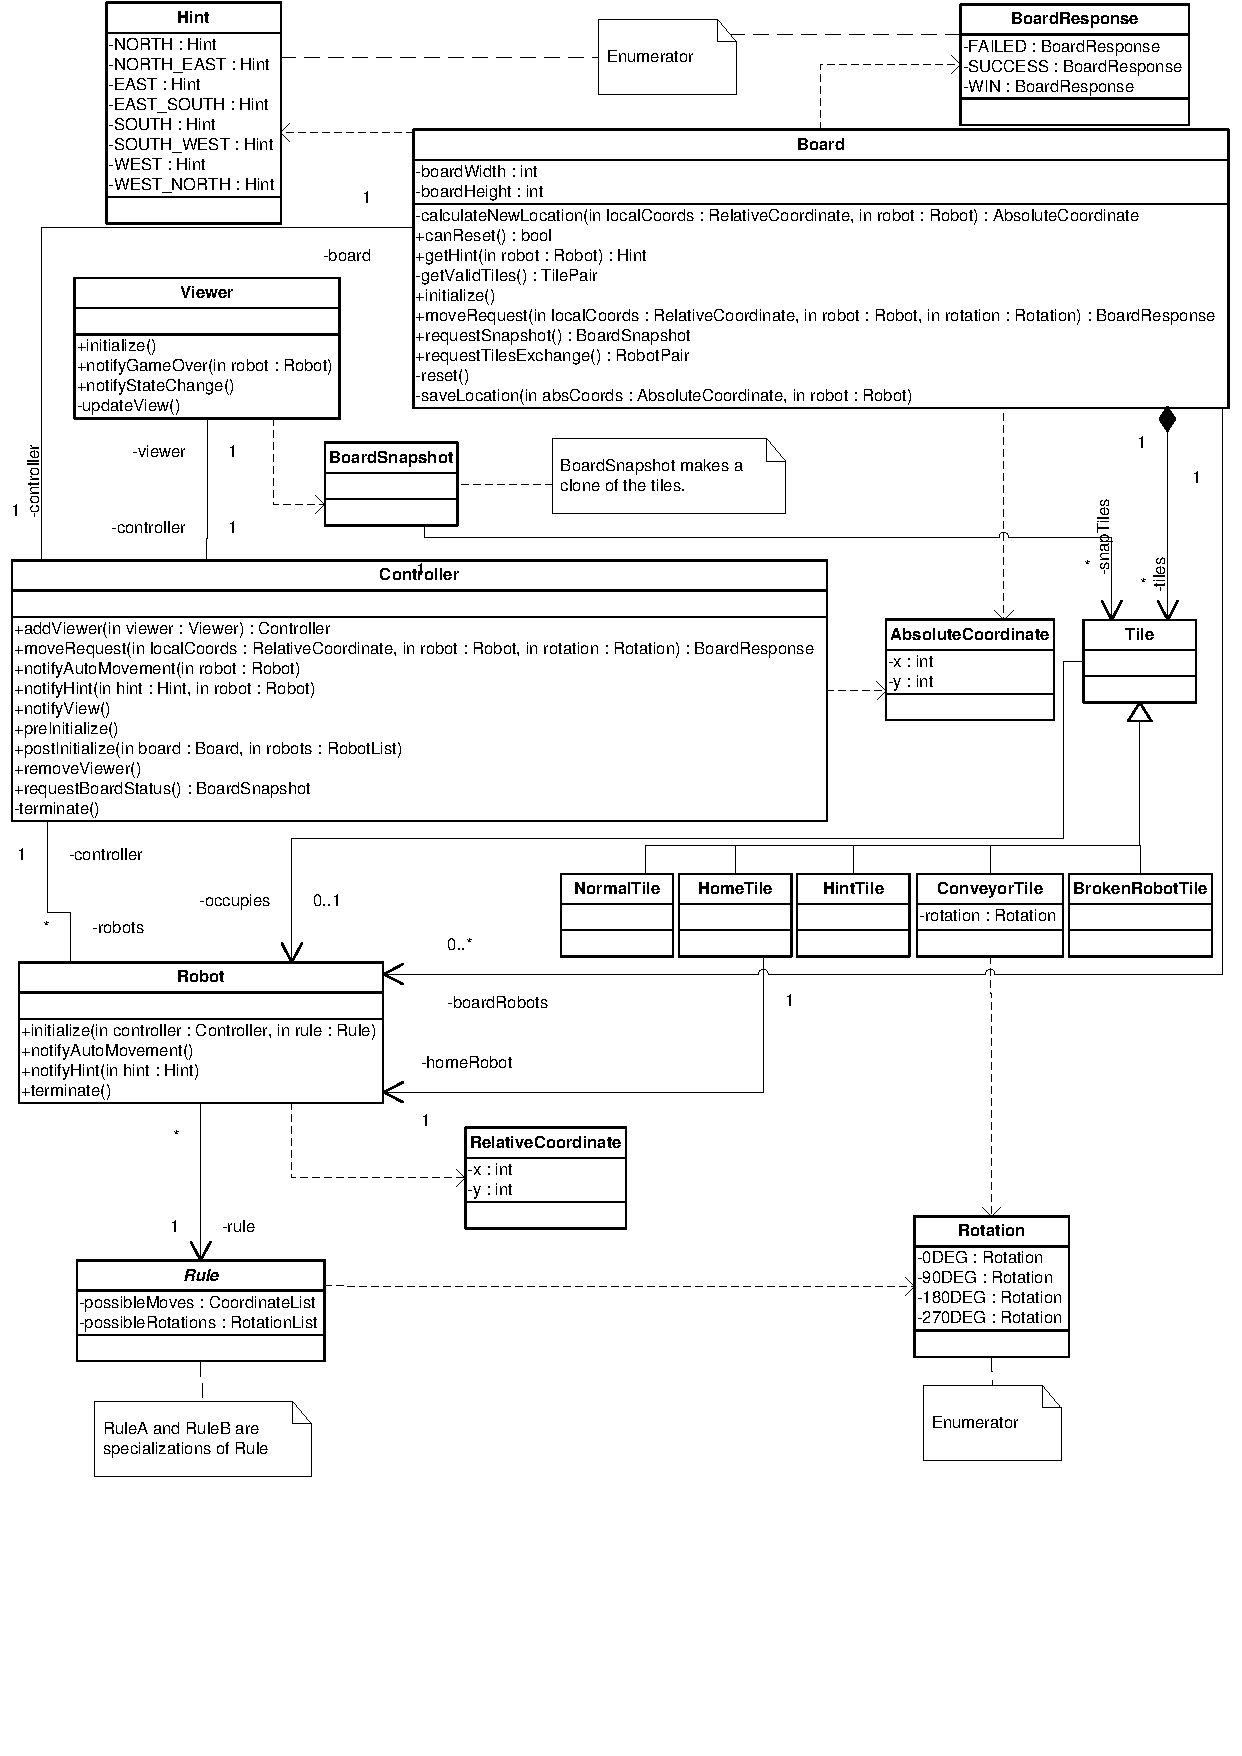
\includegraphics[width=\linewidth]{classdiagram.pdf}

\subsection{Class description}
	\begin{description}
		\item[Board] The class for the board as it was given in the informal specification.
		\item[Controller] The main controller as it was given in the informal specification.
		\item[Robot] This is used for both Robot A and Robot B in the informal sepcification.
		\item[Viewer] This is the viewer as it was given in the informal specification.
		\item[Tile] This class is used to model the tiles that the Board consists of.
		\item[NormalTile] This class is a specialization of the Tile class for a normal tile.
		\item[HomeTile] This class is a specialization of the Tile class for a home tile.
		\item[HintTile] This class is a specialization of the Tile class for a hint tile.
		\item[ConveyorTile] This class is specialization of the Tile class for a conveyor tile.
		\item[BrokenRobotTile] This class is a specialization of the Tile class for a broken robot tile.
		\item[Rule] This class is used to model the behaviour of Robot A and B in the Robot class. Any class that defines a rule inherits from this class.
		\item[Rotation] This is an enumeration class that is used to model the rotations of Robot.
		\item[RelativeCoordinate] This is a data class that contains the x and y coordinate of a relative coordinate.
		\item[AbsoluteCoordinate] This is a data class that contains the x and y coordinate of an absolute coordinate.
		\item[Hint] This in an enumeration class that contains all possible hints that a Robot can receive from a hint tile.
		\item[BoardSnapshot] This is a data class that contains a snapshot of the board, i.e. a copy of all the tiles in the board.
		\item[BoardResponse] This in an enumerator that contains all the possible responses that the board can give the controller when it makes a move request.
	\end{description}
